%%%%%%%%%%%%%%%%%%%%%%%%%%%%%%%%%%%%%%%%%%%%%%%%%%%%%%%%%%%%%%%%%%%%%%%%%%%%%%%%
% CSC2059 Practical 8
%%%%%%%%%%%%%%%%%%%%%%%%%%%%%%%%%%%%%%%%%%%%%%%%%%%%%%%%%%%%%%%%%%%%%%%%%%%%%%%%

\documentclass{csc2059practical}

% Additional packages used by this practical.
% TikZ will be used during the visual design pass.
\usepackage{tikz}
\usetikzlibrary{arrows.meta, positioning, fit, backgrounds}
\usepackage{fontawesome5}
\usepackage{booktabs}

\setpracticalnumber{8}

\setpracticaltitle{When Data Structures Shape Algorithms}

\setpracticalsubtitle{From Search Strategy to Binary Search Trees}

\setpracticalauthor{
Dr Giuseppe Trombino\\
School of Electronics, Electrical Engineering and Computer Science\\
Queen's University Belfast
}
\setpracticaldate{}

\usetikzlibrary{arrows.meta,positioning,calc}

\begin{document}

\maketitle

\tableofcontents
\clearpage

%%%%%%%%%%%%%%%%%%%%%%%%%%%%%%%%%%%%%%%%%%%%%%%%%%%%%%%%%%%%%%%%%%%%%%%%%%%%%%%%
% Introduction
%%%%%%%%%%%%%%%%%%%%%%%%%%%%%%%%%%%%%%%%%%%%%%%%%%%%%%%%%%%%%%%%%%%%%%%%%%%%%%%%

\frontsection{Introduction}

Throughout this module, you have implemented increasingly capable data
structures and the algorithms that operate on them. Arrays provided direct
access to stored values, while linked structures allowed data to grow and be
reorganised without moving every existing item.

In this practical, the focus shifts from implementing an isolated data structure
to investigating a broader engineering question:

\begin{quote}
How does the organisation of data influence the work performed by an algorithm?
\end{quote}

You will begin with a familiar linear search through a collection of books.
Rather than relying on execution time, you will count the visits and comparisons
performed by the algorithm. This gives you a stable way to compare different
search strategies and reason about where their work comes from.

You will then apply what appears to be the same search strategy to a linked
list. Before running the demonstration, you will make a prediction. The observed
result may be surprising. By tracing a small list, you will identify the source
of the unnecessary work and design a better traversal algorithm.

Improving the linked-list algorithm will remove that wasted effort, but it will
also reveal a deeper limitation: even a well-designed linear search may still
need to examine every stored item. You will therefore implement the core
recursive operations of a Binary Search Tree and investigate how a different
organisation of the same data can eliminate large parts of the remaining search
space.

The practical follows the same engineering rhythm used throughout CSC2059:

\begin{quote}
Predict $\rightarrow$ Observe $\rightarrow$ Investigate $\rightarrow$ Implement
$\rightarrow$ Measure $\rightarrow$ Explain $\rightarrow$ Reflect
\end{quote}

\begin{engineeringquestion}
When is improving an algorithm enough, and when must we reconsider the data
structure that supports it?
\end{engineeringquestion}

\begin{importantnote}
This practical is not simply about learning how to implement a Binary Search
Tree.

Its central lesson is that data structures shape algorithms, while the
operations required by an application should also shape the data structures we
choose.
\end{importantnote}
\clearpage
%%%%%%%%%%%%%%%%%%%%%%%%%%%%%%%%%%%%%%%%%%%%%%%%%%%%%%%%%%%%%%%%%%%%%%%%%%%%%%%%
% Learning Outcomes
%%%%%%%%%%%%%%%%%%%%%%%%%%%%%%%%%%%%%%%%%%%%%%%%%%%%%%%%%%%%%%%%%%%%%%%%%%%%%%%%

\begin{learningoutcomes}

By the end of this practical, you should be able to:

\begin{itemize}
    \item explain how the choice of data structure influences the work performed
          by a search algorithm;
    \item predict how different search strategies will behave before measuring
          their performance;
    \item use the \mintinline{cpp}{WorkCounter} class to compare algorithms using
          visits and comparisons rather than execution time;
    \item identify repeated work in an indexed linked-list traversal;
    \item implement and test a sequential linked-list search;
    \item implement recursive insertion and search operations for a Binary
          Search Tree;
    \item compare array, linked-list and Binary Search Tree searches using
          measured evidence;
    \item justify an appropriate data structure for the operations required by
          an application.
\end{itemize}

\end{learningoutcomes}

%%%%%%%%%%%%%%%%%%%%%%%%%%%%%%%%%%%%%%%%%%%%%%%%%%%%%%%%%%%%%%%%%%%%%%%%%%%%%%%%
% Before You Begin
%%%%%%%%%%%%%%%%%%%%%%%%%%%%%%%%%%%%%%%%%%%%%%%%%%%%%%%%%%%%%%%%%%%%%%%%%%%%%%%%

\frontsection{Before You Begin}

This practical builds on techniques and data structures developed earlier in the
module.

Before beginning, check that you can recognise the following:

\begin{itemize}
    \item cloning and opening a Classroom50 repository in Visual Studio Code;
    \item compiling programs using the supplied Makefile;
    \item running demonstrations and public Catch2 tests;
    \item interpreting a failed assertion;
    \item reading C++ classes spread across header and source files;
    \item traversing a linked list by following node pointers;
    \item using \mintinline{cpp}{nullptr} as a stopping condition;
    \item reading a simple recursive function;
    \item using a failing test to identify the next small behaviour to
          implement.
\end{itemize}

You do not need to know how a Binary Search Tree works before starting. The
practical develops that understanding from the behaviour of the search problem.
\clearpage

\begin{tipbox}
Do not run all four demonstrations immediately.

Each example is designed to answer a question raised by the previous part.
Running ahead will reveal the results before you have made the predictions and
investigated the behaviour that make those results meaningful.
\end{tipbox}

%%%%%%%%%%%%%%%%%%%%%%%%%%%%%%%%%%%%%%%%%%%%%%%%%%%%%%%%%%%%%%%%%%%%%%%%%%%%%%%%
% Repository Access
%%%%%%%%%%%%%%%%%%%%%%%%%%%%%%%%%%%%%%%%%%%%%%%%%%%%%%%%%%%%%%%%%%%%%%%%%%%%%%%%

\frontsection{Repository Access}

Access the Practical 8 repository through the link provided on Canvas, then
clone it to your local machine.

Open the cloned folder in Visual Studio Code. Do not create a separate project
or copy individual files elsewhere. The supplied Makefile expects the repository
structure to remain unchanged.

From the repository root, build the starter project:

\begin{terminal}
make
\end{terminal}

Next, run the public test suite:

\begin{terminal}
make test
\end{terminal}

The repository is supplied in a deliberate starter state. Some tests will pass
and others will fail because several functions still contain TODO markers.
Compilation should succeed, however.

The four demonstrations can be run using:

\begin{terminal}
make run-example01
make run-example02
make run-example03
make run-example04
\end{terminal}

Run each demonstration only when directed by the guide.

Throughout the practical:

\begin{itemize}
    \item make a prediction before observing a result;
    \item investigate one behaviour at a time;
    \item study the relevant public tests before implementing a function;
    \item rerun the tests after each small change;
    \item keep previously passing tests green;
    \item commit and push regularly using meaningful messages.
\end{itemize}

%%%%%%%%%%%%%%%%%%%%%%%%%%%%%%%%%%%%%%%%%%%%%%%%%%%%%%%%%%%%%%%%%%%%%%%%%%%%%%%%
% Repository Tour
%%%%%%%%%%%%%%%%%%%%%%%%%%%%%%%%%%%%%%%%%%%%%%%%%%%%%%%%%%%%%%%%%%%%%%%%%%%%%%%%

\frontsection{Repository Tour}

The repository is organised around four demonstrations and the implementations
they motivate.

\begin{center}
\begin{tabular}{p{0.34\textwidth} p{0.58\textwidth}}
\toprule
\textbf{Path} & \textbf{Purpose} \\
\midrule
\texttt{examples/} & Demonstrations used to observe and compare search
                      behaviour. \\
\texttt{include/} & Public interfaces and template implementations. \\
\texttt{src/} & Search algorithms, supporting classes and starter
                  implementations. \\
\texttt{tests/} & Public Catch2 tests that guide each implementation step. \\
\texttt{data/} & Book datasets used by the demonstrations. \\
\texttt{external/} & The supplied Catch2 testing framework. \\
\texttt{bin/} & Generated executables created by the Makefile. \\
\texttt{Makefile} & Builds and runs demonstrations and tests. \\
\texttt{README.md} & A concise repository survival guide. \\
\bottomrule
\end{tabular}
\end{center}

The demonstrations form a deliberate progression:

\begin{center}
\begin{tabular}{p{0.34\textwidth} p{0.58\textwidth}}
\toprule
\textbf{Example} & \textbf{Purpose} \\
\midrule
\texttt{example01}
&
Establishes the baseline cost of a linear array search and introduces the work
counter.
\\[1mm]

\texttt{example02}
&
Reveals the repeated work caused by accessing a linked list through indexed
positions.
\\[1mm]

\texttt{example03}
&
Confirms that a direct sequential traversal removes the unnecessary repeated
visits.
\\[1mm]

\texttt{example04}
&
Compares all four searches and demonstrates how a Binary Search Tree can reduce
the remaining search work.
\\
\bottomrule
\end{tabular}
\end{center}

The practical follows this engineering journey:

\begin{center}
\begin{tabular}{p{0.12\textwidth} p{0.76\textwidth}}
\toprule
\textbf{Part} & \textbf{Engineering Journey} \\
\midrule
A & Establish a reliable way to measure algorithmic work. \\
B & Predict, observe and investigate an unexpectedly expensive linked-list
    search. \\
C & Implement a sequential traversal and restore the search to the linear
    baseline. \\
D & Implement Binary Search Tree operations and compare all four approaches. \\
\bottomrule
\end{tabular}
\end{center}

%%%%%%%%%%%%%%%%%%%%%%%%%%%%%%%%%%%%%%%%%%%%%%%%%%%%%%%%%%%%%%%%%%%%%%%%%%%%%%%%
% Thinking Like an Engineer
%%%%%%%%%%%%%%%%%%%%%%%%%%%%%%%%%%%%%%%%%%%%%%%%%%%%%%%%%%%%%%%%%%%%%%%%%%%%%%%%

\frontsection{Thinking Like an Engineer}

Suppose an application stores 10,000 books and must find one using its
identifier.

Before running any demonstrations, record the following predictions in your own
notes:

\begin{itemize}
    \item How much work might a linear array search perform?
    \item Would searching a linked list require less work, more work or about
          the same amount?
    \item How might a Binary Search Tree change the search?
\end{itemize}

For each prediction, write one or two sentences explaining your reasoning.

Do not worry about being correct at this stage. A useful prediction is one that
can later be compared with evidence.

Return to these notes as you work through the practical. Where the observed
behaviour differs from your prediction, investigate why.

\begin{reflectionbox}
What assumptions are you making about how each data structure is searched?

Could two different algorithms operating on the same data structure perform
very different amounts of work?
\end{reflectionbox}

%%%%%%%%%%%%%%%%%%%%%%%%%%%%%%%%%%%%%%%%%%%%%%%%%%%%%%%%%%%%%%%%%%%%%%%%%%%%%%%%
% Suggested Workflow
%%%%%%%%%%%%%%%%%%%%%%%%%%%%%%%%%%%%%%%%%%%%%%%%%%%%%%%%%%%%%%%%%%%%%%%%%%%%%%%%

\frontsection{A Suggested Workflow}

Throughout this practical, use the following process:

\begin{enumerate}
    \item \textbf{Predict} what you expect to happen and explain why.
    \item \textbf{Observe} the evidence produced by a demonstration or test.
    \item \textbf{Investigate} where the measured work comes from.
    \item \textbf{Implement} one small improvement at a time.
    \item \textbf{Measure} the behaviour again.
    \item \textbf{Explain} why the result changed.
    \item \textbf{Reflect} on whether the remaining limitation belongs to the
          algorithm or to the data structure.
\end{enumerate}

The aim is not simply to make the tests pass. Each implementation should answer
an engineering question raised by the evidence you have already observed.
\clearpage
\begin{importantnote}
Do not change a data structure merely because one algorithm performs badly.

First determine whether the structure is being used appropriately. Once the
algorithm has been improved, ask whether the remaining work is an unavoidable
property of that structure.
\end{importantnote}

%%%%%%%%%%%%%%%%%%%%%%%%%%%%%%%%%%%%%%%%%%%%%%%%%%%%%%%%%%%%%%%%%%%%%%%%%%%%%%%%
% Part A begins here
%%%%%%%%%%%%%%%%%%%%%%%%%%%%%%%%%%%%%%%%%%%%%%%%%%%%%%%%%%%%%%%%%%%%%%%%%%%%%%%%

% \section{Part A --- Measuring Work Instead of Time}

%%%%%%%%%%%%%%%%%%%%%%%%%%%%%%%%%%%%%%%%%%%%%%%%%%%%%%%%%%%%%%%%%%%%%%%%%%%%%%%%
% Part A --- Measuring Work Instead of Time
%%%%%%%%%%%%%%%%%%%%%%%%%%%%%%%%%%%%%%%%%%%%%%%%%%%%%%%%%%%%%%%%%%%%%%%%%%%%%%%%

\section{Part A --- Measuring Work Instead of Time}


\begin{infobox}[Estimated Effort]
Estimated time: approx \textbf{10 minutes}
\end{infobox}


\begin{engineeringquestion}
If computers run at different speeds, how can we compare two algorithms fairly?
\end{engineeringquestion}

When software engineers compare algorithms, execution time alone is rarely a
reliable measurement. The same program may take different amounts of time
depending on the processor, operating system, compiler settings and other
programs running on the computer.

Instead, we can examine the amount of \emph{work} performed by an algorithm.

For a search algorithm, two useful measurements are:

\begin{description}
    \item[Visits] The number of stored items or nodes examined by the algorithm.
    \item[Comparisons] The number of times a stored value is compared with the
          target value.
\end{description}

These measurements allow us to compare algorithms independently of the machine
on which they are executed.

Throughout this practical, the supplied \mintinline{cpp}{WorkCounter} class
records this information for each search.

%%%%%%%%%%%%%%%%%%%%%%%%%%%%%%%%%%%%%%%%%%%%%%%%%%%%%%%%%%%%%%%%%%%%%%%%%%%%%%%%
% Investigating the Measurement Classes
%%%%%%%%%%%%%%%%%%%%%%%%%%%%%%%%%%%%%%%%%%%%%%%%%%%%%%%%%%%%%%%%%%%%%%%%%%%%%%%%

\subsection{Investigating the Measurement Classes}

Before running the first demonstration, locate the files that define:

\begin{itemize}
    \item \mintinline{cpp}{WorkCounter}
    \item \mintinline{cpp}{SearchResult}
\end{itemize}

Read their public interfaces and answer the following questions in your own
notes:

\begin{enumerate}
    \item What information is recorded by \mintinline{cpp}{WorkCounter}?
    \item What information is returned in a \mintinline{cpp}{SearchResult}?
    \item Why might visits and comparisons be more useful than measuring
          execution time?
\end{enumerate}

You do not need to understand every implementation detail. Concentrate on the
information these classes allow a search algorithm to report.

%%%%%%%%%%%%%%%%%%%%%%%%%%%%%%%%%%%%%%%%%%%%%%%%%%%%%%%%%%%%%%%%%%%%%%%%%%%%%%%%
% Establishing a Baseline
%%%%%%%%%%%%%%%%%%%%%%%%%%%%%%%%%%%%%%%%%%%%%%%%%%%%%%%%%%%%%%%%%%%%%%%%%%%%%%%%

\subsection{Establishing a Baseline}

The first demonstration performs a linear search through the application dataset.

The target book has deliberately been selected from the end of the collection.
Before running the demonstration, make a prediction:

\begin{reflectionbox}
The dataset contains 10,000 books.

How many books do you expect a linear search to visit before finding the final
book?

How many identifier comparisons do you expect it to perform?
\end{reflectionbox}

Now run the first demonstration:

\begin{terminal}
make example01
\end{terminal}

Your output should report that the target was found and display the work
performed by the search.

You should observe approximately:

\begin{terminal}
Visits: 10000
Comparisons: 10000
\end{terminal}

%%%%%%%%%%%%%%%%%%%%%%%%%%%%%%%%%%%%%%%%%%%%%%%%%%%%%%%%%%%%%%%%%%%%%%%%%%%%%%%%
% Observation
%%%%%%%%%%%%%%%%%%%%%%%%%%%%%%%%%%%%%%%%%%%%%%%%%%%%%%%%%%%%%%%%%%%%%%%%%%%%%%%%

\subsection{Observation}

The linear search begins with the first book and examines each entry in order
until the target is found.

Because the target is the final book in the dataset, the algorithm must visit
all 10,000 books. Each visit also requires the stored identifier to be compared
with the target identifier.

The search therefore performs:

\begin{itemize}
    \item 10,000 visits;
    \item 10,000 comparisons.
\end{itemize}

This result establishes the \emph{baseline} that will be used throughout the
remainder of the practical.

\begin{importantnote}
The purpose of the work counter is not to decide that 10,000 operations are
automatically ``good'' or ``bad''.

It gives us a consistent measurement that can be compared with the work
performed by other search algorithms using the same dataset and target.
\end{importantnote}

%%%%%%%%%%%%%%%%%%%%%%%%%%%%%%%%%%%%%%%%%%%%%%%%%%%%%%%%%%%%%%%%%%%%%%%%%%%%%%%%
% Engineering Takeaway
%%%%%%%%%%%%%%%%%%%%%%%%%%%%%%%%%%%%%%%%%%%%%%%%%%%%%%%%%%%%%%%%%%%%%%%%%%%%%%%%

\subsection{Engineering Takeaway}

Execution time may change from one computer or one run to another. Counting the
operations performed by an algorithm gives us a more stable basis for comparison.

We now have:

\begin{itemize}
    \item a dataset containing 10,000 books;
    \item a target stored at the end of that dataset;
    \item a linear-search baseline of 10,000 visits and 10,000 comparisons;
    \item a consistent way to measure the work performed by later searches.
\end{itemize}

In Part B, you will use the same measurement process to investigate a search
through a linked list.

Before seeing the result, however, you will need to predict what you expect to
happen.

%%%%%%%%%%%%%%%%%%%%%%%%%%%%%%%%%%%%%%%%%%%%%%%%%%%%%%%%%%%%%%%%%%%%%%%%%%%%%%%%
% Part B --- When Familiar Code Performs Unexpected Work
%%%%%%%%%%%%%%%%%%%%%%%%%%%%%%%%%%%%%%%%%%%%%%%%%%%%%%%%%%%%%%%%%%%%%%%%%%%%%%%%

\section{Part B --- When Familiar Code Performs Unexpected Work}


\begin{infobox}[Estimated Effort]
Estimated time: approx \textbf{20 minutes}
\end{infobox}


\begin{engineeringquestion}
If an array and a linked list contain the same 10,000 books, should searching
them require approximately the same amount of work?
\end{engineeringquestion}

In Part A, the linear array search established a baseline of:

\begin{itemize}
    \item 10,000 visits;
    \item 10,000 comparisons.
\end{itemize}

The repository also contains a search that examines the same books after they
have been stored in a linked list.

The search still examines the books in order, beginning with the first item and
continuing until it finds the target. It may therefore appear reasonable to
expect behaviour similar to the array search.

Do not run the second demonstration yet.

%%%%%%%%%%%%%%%%%%%%%%%%%%%%%%%%%%%%%%%%%%%%%%%%%%%%%%%%%%%%%%%%%%%%%%%%%%%%%%%%
% Make a Prediction
%%%%%%%%%%%%%%%%%%%%%%%%%%%%%%%%%%%%%%%%%%%%%%%%%%%%%%%%%%%%%%%%%%%%%%%%%%%%%%%%

\subsection{Make a Prediction}

The linked list contains the same 10,000 books as the array, in the same order.
The target is again the final book.

In your own notes, predict the result of the linked-list search.

\begin{reflectionbox}
Do you expect the linked-list search to perform:

\begin{itemize}
    \item fewer than 10,000 visits;
    \item approximately 10,000 visits; or
    \item more than 10,000 visits?
\end{itemize}

How many comparisons do you expect?

Write one or two sentences explaining your reasoning before continuing.
\end{reflectionbox}

%%%%%%%%%%%%%%%%%%%%%%%%%%%%%%%%%%%%%%%%%%%%%%%%%%%%%%%%%%%%%%%%%%%%%%%%%%%%%%%%
% Observe the Result
%%%%%%%%%%%%%%%%%%%%%%%%%%%%%%%%%%%%%%%%%%%%%%%%%%%%%%%%%%%%%%%%%%%%%%%%%%%%%%%%

\subsection{Observe the Result}

Now run the second demonstration:

\begin{terminal}
make example02
\end{terminal}

The demonstration compares the original linear array search with a linked-list
search that accesses the list using indexed positions.

You should observe results similar to:

\begin{terminal}
Linear Array Search
Visits: 10000
Comparisons: 10000

Indexed Linked-List Search
Visits: 50005000
Comparisons: 10000
\end{terminal}

The linked-list search performs the expected 10,000 comparisons.

However, it performs more than 50 million node visits.

\begin{reflectionbox}
How closely did this result match your prediction?

Why might the number of comparisons remain at 10,000 while the number of visits
increases so dramatically?
\end{reflectionbox}

Do not move directly to the next example. The purpose of this part is to explain
where those additional visits come from.

%%%%%%%%%%%%%%%%%%%%%%%%%%%%%%%%%%%%%%%%%%%%%%%%%%%%%%%%%%%%%%%%%%%%%%%%%%%%%%%%
% Investigate the Search
%%%%%%%%%%%%%%%%%%%%%%%%%%%%%%%%%%%%%%%%%%%%%%%%%%%%%%%%%%%%%%%%%%%%%%%%%%%%%%%%

\subsection{Investigate the Search}

Open:

\begin{terminal}
examples/example02_indexed_list_search.cpp
\end{terminal}

Follow the function calls until you locate the linked-list search used by the
demonstration.

Read the implementation carefully.

Look for the operation used to retrieve each book from the list.

\begin{importantnote}
An array can access an indexed position directly.

A linked list cannot jump immediately to an arbitrary node. To reach a position,
it must begin at the head and follow the links between nodes.
\end{importantnote}

The search may resemble a conventional indexed loop, but the cost of accessing
each position is very different from indexed access to an array.

%%%%%%%%%%%%%%%%%%%%%%%%%%%%%%%%%%%%%%%%%%%%%%%%%%%%%%%%%%%%%%%%%%%%%%%%%%%%%%%%
% Trace a Five-Node List
%%%%%%%%%%%%%%%%%%%%%%%%%%%%%%%%%%%%%%%%%%%%%%%%%%%%%%%%%%%%%%%%%%%%%%%%%%%%%%%%

\subsection{Trace a Five-Node List}

Consider a linked list containing five books:

\begin{center}
\texttt{Book 0}
$\longrightarrow$
\texttt{Book 1}
$\longrightarrow$
\texttt{Book 2}
$\longrightarrow$
\texttt{Book 3}
$\longrightarrow$
\texttt{Book 4}
\end{center}

Assume that the target is stored in the final node.

The indexed search requests each position separately:

\begin{center}
\begin{tabular}{c c c}
\toprule
\textbf{Requested position} &
\textbf{Nodes visited to reach it} &
\textbf{Visits performed} \\
\midrule
0 & Book 0 & 1 \\
1 & Book 0 $\rightarrow$ Book 1 & 2 \\
2 & Book 0 $\rightarrow$ Book 1 $\rightarrow$ Book 2 & 3 \\
3 & Book 0 $\rightarrow$ Book 1 $\rightarrow$ Book 2
  $\rightarrow$ Book 3 & 4 \\
4 & Book 0 $\rightarrow$ Book 1 $\rightarrow$ Book 2
  $\rightarrow$ Book 3 $\rightarrow$ Book 4 & 5 \\
\bottomrule
\end{tabular}
\end{center}

The five comparisons require:

\[
1 + 2 + 3 + 4 + 5 = 15
\]

node visits.

Complete the same reasoning in your own notes for a list containing six nodes.


\begin{reflectionbox}
When the search requests the next indexed position, which nodes are visited
again?

How much of the previous traversal is discarded and repeated?
\end{reflectionbox}


\begin{figure}[htbp]
    \centering

    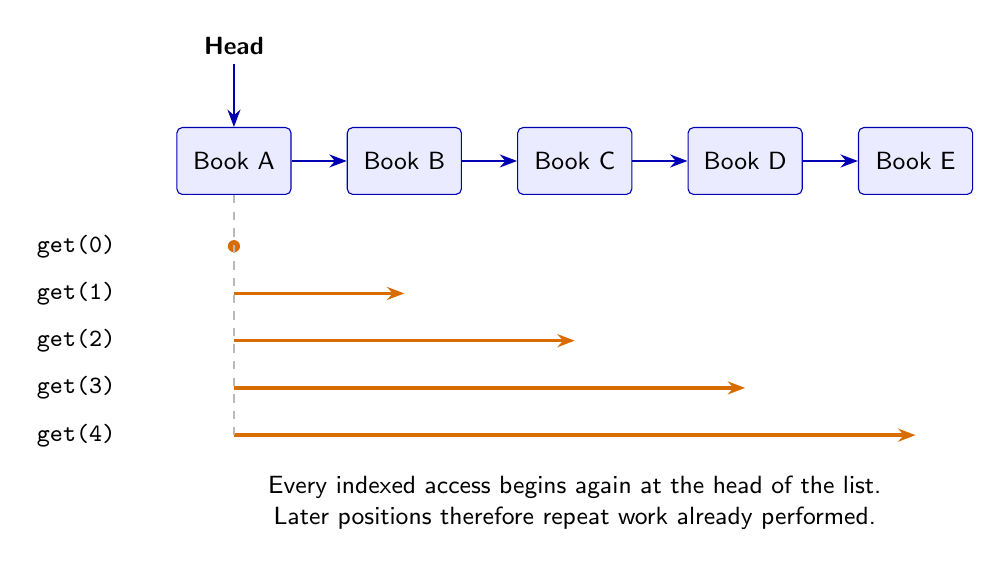
\begin{tikzpicture}[
        node distance=0.7cm,
        dataNode/.style={
            draw=blue!70!black,
            fill=blue!8,
            rounded corners=2pt,
            minimum width=1.45cm,
            minimum height=0.85cm,
            font=\sffamily\small
        },
        pointer/.style={
            -{Stealth[length=2.2mm]},
            thick,
            draw=blue!70!black
        },
        traversal/.style={
            -{Stealth[length=2.2mm]},
            very thick,
            draw=orange!85!black
        },
        labelText/.style={
            font=\sffamily\small,
            anchor=east
        }
    ]

        % Linked-list nodes
        \node[dataNode] (a) {Book A};
        \node[dataNode, right=of a] (b) {Book B};
        \node[dataNode, right=of b] (c) {Book C};
        \node[dataNode, right=of c] (d) {Book D};
        \node[dataNode, right=of d] (e) {Book E};

        % List pointers
        \draw[pointer] (a) -- (b);
        \draw[pointer] (b) -- (c);
        \draw[pointer] (c) -- (d);
        \draw[pointer] (d) -- (e);

        % Head pointer
        \node[
            font=\sffamily\bfseries\small,
            above=0.8cm of a
        ] (head) {Head};

        \draw[pointer] (head) -- (a);

        % Traversal labels
        \node[labelText] (label0)
            at ($(a.south west)+(-0.65,-0.65)$)
            {\texttt{get(0)}};

        \node[labelText] (label1)
            at ($(a.south west)+(-0.65,-1.25)$)
            {\texttt{get(1)}};

        \node[labelText] (label2)
            at ($(a.south west)+(-0.65,-1.85)$)
            {\texttt{get(2)}};

        \node[labelText] (label3)
            at ($(a.south west)+(-0.65,-2.45)$)
            {\texttt{get(3)}};

        \node[labelText] (label4)
            at ($(a.south west)+(-0.65,-3.05)$)
            {\texttt{get(4)}};

        % Repeated traversals
        \fill[orange!85!black]
            ($(a.south)+(0,-0.65)$)
            circle[radius=2.2pt];

        \draw[traversal]
            ($(a.south)+(0,-1.25)$)
            --
            ($(b.south)+(0,-1.25)$);

        \draw[traversal]
            ($(a.south)+(0,-1.85)$)
            --
            ($(c.south)+(0,-1.85)$);

        \draw[traversal]
            ($(a.south)+(0,-2.45)$)
            --
            ($(d.south)+(0,-2.45)$);

        \draw[traversal]
            ($(a.south)+(0,-3.05)$)
            --
            ($(e.south)+(0,-3.05)$);

        % Starting-point guides
        \foreach \offset in {0.65,1.25,1.85,2.45,3.05}
        {
            \draw[
                dashed,
                draw=gray!55
            ]
            (a.south)
            --
            ($(a.south)+(0,-\offset)$);
        }

        % Explanatory annotation
        \node[
            font=\sffamily\small,
            text width=8.5cm,
            align=center,
            below=3.45cm of c
        ] {
            Every indexed access begins again at the head of the list.
            Later positions therefore repeat work already performed.
        };

    \end{tikzpicture}

    \caption{
        Indexed access repeatedly traverses the linked list from its head.
    }
    \label{fig:indexed-list-repeated-traversal}
\end{figure}

%%%%%%%%%%%%%%%%%%%%%%%%%%%%%%%%%%%%%%%%%%%%%%%%%%%%%%%%%%%%%%%%%%%%%%%%%%%%%%%%
% Explain the Application Result
%%%%%%%%%%%%%%%%%%%%%%%%%%%%%%%%%%%%%%%%%%%%%%%%%%%%%%%%%%%%%%%%%%%%%%%%%%%%%%%%

\subsection{Explain the Application Result}

For a list containing 10,000 books, the indexed search performs:

\[
1 + 2 + 3 + \cdots + 10{,}000
\]

node visits.

This produces the measured result:

\[
50{,}005{,}000
\]

The search still compares each of the 10,000 books with the target only once.
The extra work comes from repeatedly travelling from the head of the list to
reach each indexed position.

The problem is therefore not that linked lists inherently require 50 million
visits to search 10,000 books.

The problem is the way this algorithm uses the linked list.

\begin{importantnote}
Source code that looks familiar does not necessarily perform familiar work.

An indexed loop is natural for an array because indexed access is direct. The
same loop applied to a linked list can repeatedly traverse nodes that have
already been visited.
\end{importantnote}

%%%%%%%%%%%%%%%%%%%%%%%%%%%%%%%%%%%%%%%%%%%%%%%%%%%%%%%%%%%%%%%%%%%%%%%%%%%%%%%%
% Design an Improvement
%%%%%%%%%%%%%%%%%%%%%%%%%%%%%%%%%%%%%%%%%%%%%%%%%%%%%%%%%%%%%%%%%%%%%%%%%%%%%%%%

\subsection{Design an Improvement}

The indexed search repeatedly returns to the head of the list.

Consider how you would search the same list manually.

After examining the first node, would you return to the beginning before
examining the second node?

In your own notes, describe an alternative search algorithm that:

\begin{itemize}
    \item begins at the head of the list;
    \item examines the current node;
    \item moves directly to the next node;
    \item never returns to the head unnecessarily;
    \item stops when the target is found or the end of the list is reached.
\end{itemize}

You do not need to write C++ code yet. First describe the algorithm in plain
language or pseudocode.

\begin{reflectionbox}
For the five-node example, how many visits would your improved algorithm
perform?

For the 10,000-book dataset, what result do you now predict?
\end{reflectionbox}

%%%%%%%%%%%%%%%%%%%%%%%%%%%%%%%%%%%%%%%%%%%%%%%%%%%%%%%%%%%%%%%%%%%%%%%%%%%%%%%%
% Engineering Takeaway
%%%%%%%%%%%%%%%%%%%%%%%%%%%%%%%%%%%%%%%%%%%%%%%%%%%%%%%%%%%%%%%%%%%%%%%%%%%%%%%%

\subsection{Engineering Takeaway}

The indexed linked-list search performed an enormous amount of unnecessary work,
but the data structure itself was not yet the problem.

The algorithm treated indexed access to a linked list as though it were indexed
access to an array. Each request began another traversal from the head, causing
earlier nodes to be visited repeatedly.

Before replacing a data structure, an engineer should first ask:

\begin{quote}
Are we using the current data structure appropriately?
\end{quote}

In Part C, you will turn your proposed improvement into a sequential
linked-list search and use the work counter to determine whether it removes the
repeated traversal.

%%%%%%%%%%%%%%%%%%%%%%%%%%%%%%%%%%%%%%%%%%%%%%%%%%%%%%%%%%%%%%%%%%%%%%%%%%%%%%%%
% Part C --- Eliminating the Repeated Work
%%%%%%%%%%%%%%%%%%%%%%%%%%%%%%%%%%%%%%%%%%%%%%%%%%%%%%%%%%%%%%%%%%%%%%%%%%%%%%%%

\section{Part C --- Eliminating the Repeated Work}


\begin{infobox}[Estimated Effort]
Estimated time: approx \textbf{30 minutes}
\end{infobox}


\begin{engineeringquestion}
Can we search a linked list efficiently without repeatedly returning to the
head of the list?
\end{engineeringquestion}

In Part B, you discovered that the poor performance of the indexed linked-list
search was not caused by the linked list itself. Instead, the search repeatedly
started a new traversal from the head of the list every time it requested the
next indexed position.

Before replacing a data structure, good software engineers first ask whether
the existing algorithm can be improved.

In this part, you will implement the sequential traversal you designed in
Part B and use the public tests to verify that it removes the unnecessary
repeated work.

%%%%%%%%%%%%%%%%%%%%%%%%%%%%%%%%%%%%%%%%%%%%%%%%%%%%%%%%%%%%%%%%%%%%%%%%%%%%%%%%
% Inspect the Public Tests
%%%%%%%%%%%%%%%%%%%%%%%%%%%%%%%%%%%%%%%%%%%%%%%%%%%%%%%%%%%%%%%%%%%%%%%%%%%%%%%%

\subsection{Inspect the Public Tests}

Before writing any code, examine the new public test file:

\begin{terminal}
tests/test02_sequential_list_search.cpp
\end{terminal}

Notice that the tests gradually build the required behaviour.

They check that your search correctly handles:

\begin{itemize}
    \item an empty linked list;
    \item a target stored at the beginning of the list;
    \item a target stored in the middle of the list;
    \item a target stored at the end of the list;
    \item a missing target.
\end{itemize}

The final test also measures the amount of work performed by your algorithm.

Unlike the indexed search from Part B, a correct sequential traversal should
visit each node only once.

%%%%%%%%%%%%%%%%%%%%%%%%%%%%%%%%%%%%%%%%%%%%%%%%%%%%%%%%%%%%%%%%%%%%%%%%%%%%%%%%
% Implement the Search
%%%%%%%%%%%%%%%%%%%%%%%%%%%%%%%%%%%%%%%%%%%%%%%%%%%%%%%%%%%%%%%%%%%%%%%%%%%%%%%%

\subsection{Implement the Search}

Open:

\begin{terminal}
src/SearchAlgorithms.cpp
\end{terminal}

Locate the function:

\begin{terminal}
sequentialListSearchById(...)
\end{terminal}

The function currently contains a TODO marker.

Implement the sequential search algorithm you designed in Part B.

Remember that a sequential traversal should:

\begin{itemize}
    \item begin at the head of the list;
    \item examine the current book;
    \item compare its identifier with the target identifier;
    \item move directly to the next node;
    \item stop when the book is found or the end of the list is reached.
\end{itemize}

Avoid accessing the linked list through indexed positions.

Doing so would recreate the inefficient behaviour investigated in Part B.

%%%%%%%%%%%%%%%%%%%%%%%%%%%%%%%%%%%%%%%%%%%%%%%%%%%%%%%%%%%%%%%%%%%%%%%%%%%%%%%%
% Test Your Implementation
%%%%%%%%%%%%%%%%%%%%%%%%%%%%%%%%%%%%%%%%%%%%%%%%%%%%%%%%%%%%%%%%%%%%%%%%%%%%%%%%

\subsection{Test Your Implementation}

Compile and run only the Part C tests:

\begin{terminal}
make test-part-c
\end{terminal}

Initially, several tests should fail.

Implement your solution one small step at a time, rerunning the tests after
each improvement.

Continue until every Part C test passes successfully.

\begin{tipbox}
Resist the temptation to write the entire function before testing it.

A small implementation followed by a successful test provides much clearer
feedback than attempting to solve everything in one attempt.
\end{tipbox}

%%%%%%%%%%%%%%%%%%%%%%%%%%%%%%%%%%%%%%%%%%%%%%%%%%%%%%%%%%%%%%%%%%%%%%%%%%%%%%%%
% Compare the Results
%%%%%%%%%%%%%%%%%%%%%%%%%%%%%%%%%%%%%%%%%%%%%%%%%%%%%%%%%%%%%%%%%%%%%%%%%%%%%%%%

\subsection{Compare the Results}

Now run the third demonstration:

\begin{terminal}
make example03
\end{terminal}

The demonstration compares the original linear array search with your new
sequential linked-list search.

You should observe results similar to:

\begin{terminal}
Linear Array Search
Visits: 10000
Comparisons: 10000

Sequential Linked-List Search
Visits: 10000
Comparisons: 10000
\end{terminal}

%%%%%%%%%%%%%%%%%%%%%%%%%%%%%%%%%%%%%%%%%%%%%%%%%%%%%%%%%%%%%%%%%%%%%%%%%%%%%%%%
% Observation
%%%%%%%%%%%%%%%%%%%%%%%%%%%%%%%%%%%%%%%%%%%%%%%%%%%%%%%%%%%%%%%%%%%%%%%%%%%%%%%%

\subsection{Observation}

Your new search has eliminated the repeated traversal that produced over
50 million node visits in Part B.

The linked-list search now performs approximately the same amount of work as
the original linear array search.

This confirms that the excessive work observed earlier was caused by the
algorithm rather than by the linked-list data structure itself.

\begin{figure}[htbp]
    \centering

    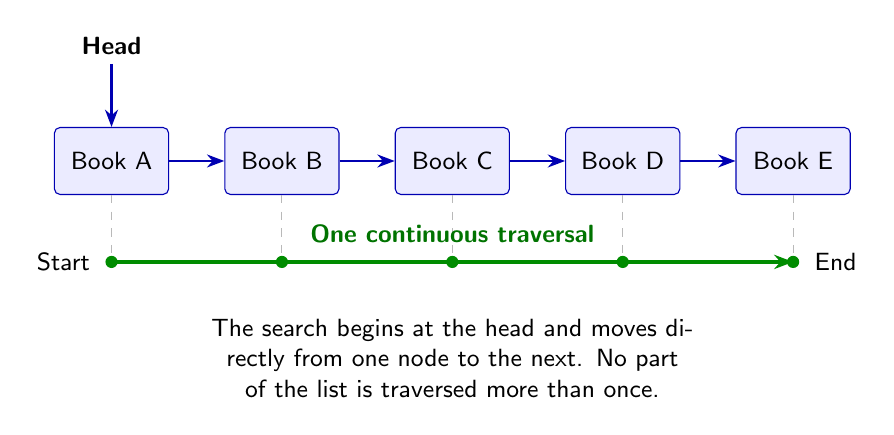
\begin{tikzpicture}[
        node distance=0.7cm,
        dataNode/.style={
            draw=blue!70!black,
            fill=blue!8,
            rounded corners=2pt,
            minimum width=1.45cm,
            minimum height=0.85cm,
            font=\sffamily\small
        },
        pointer/.style={
            -{Stealth[length=2.2mm]},
            thick,
            draw=blue!70!black
        },
        traversal/.style={
            -{Stealth[length=2.4mm]},
            very thick,
            draw=green!55!black
        }
    ]

        % Linked-list nodes
        \node[dataNode] (a) {Book A};
        \node[dataNode, right=of a] (b) {Book B};
        \node[dataNode, right=of b] (c) {Book C};
        \node[dataNode, right=of c] (d) {Book D};
        \node[dataNode, right=of d] (e) {Book E};

        % List pointers
        \draw[pointer] (a) -- (b);
        \draw[pointer] (b) -- (c);
        \draw[pointer] (c) -- (d);
        \draw[pointer] (d) -- (e);

        % Head pointer
        \node[
            font=\sffamily\bfseries\small,
            above=0.8cm of a
        ] (head) {Head};

        \draw[pointer] (head) -- (a);

        % Sequential traversal path
        \coordinate (start) at ($(a.south)+(0,-0.85)$);
        \coordinate (finish) at ($(e.south)+(0,-0.85)$);

        \draw[traversal]
            (start)
            --
            (finish);

        % Mark each node visit
        \foreach \nodeName in {a,b,c,d,e}
        {
            \draw[
                dashed,
                draw=gray!55
            ]
            (\nodeName.south)
            --
            ($(\nodeName.south)+(0,-0.85)$);

            \fill[
                green!55!black
            ]
            ($(\nodeName.south)+(0,-0.85)$)
            circle[radius=2.2pt];
        }

        % Start and finish labels
        \node[
            font=\sffamily\small,
            anchor=east
        ]
        at ($(start)+(-0.15,0)$)
        {Start};

        \node[
            font=\sffamily\small,
            anchor=west
        ]
        at ($(finish)+(0.15,0)$)
        {End};

        % Traversal annotation
        \node[
            font=\sffamily\bfseries\small,
            text=green!45!black,
            above=0.12cm
        ]
        at ($(start)!0.5!(finish)$)
        {One continuous traversal};

        % Explanatory annotation
        \node[
            font=\sffamily\small,
            text width=8.5cm,
            align=center,
            below=1.45cm of c
        ] {
            The search begins at the head and moves directly from one node
            to the next. No part of the list is traversed more than once.
        };

    \end{tikzpicture}

    \caption{
        Sequential traversal examines each linked-list node at most once.
    }
    \label{fig:sequential-list-traversal}
\end{figure}


%%%%%%%%%%%%%%%%%%%%%%%%%%%%%%%%%%%%%%%%%%%%%%%%%%%%%%%%%%%%%%%%%%%%%%%%%%%%%%%%
% Reflection
%%%%%%%%%%%%%%%%%%%%%%%%%%%%%%%%%%%%%%%%%%%%%%%%%%%%%%%%%%%%%%%%%%%%%%%%%%%%%%%%

\subsection{Reflection}

Although the sequential traversal removes the unnecessary repeated visits, the
search still performs approximately 10,000 comparisons when the target is
stored at the end of the dataset.

\begin{reflectionbox}
Your algorithm is now using the linked list efficiently.

Where do the remaining 10,000 comparisons come from?

If the algorithm is no longer wasting work, could a different organisation of
the data reduce the amount of searching still further?
\end{reflectionbox}

%%%%%%%%%%%%%%%%%%%%%%%%%%%%%%%%%%%%%%%%%%%%%%%%%%%%%%%%%%%%%%%%%%%%%%%%%%%%%%%%
% Engineering Takeaway
%%%%%%%%%%%%%%%%%%%%%%%%%%%%%%%%%%%%%%%%%%%%%%%%%%%%%%%%%%%%%%%%%%%%%%%%%%%%%%%%

\subsection{Engineering Takeaway}

The first instinct when software performs poorly is often to replace the data
structure.

This practical has shown that a better question is:

\begin{quote}
Are we using the current data structure appropriately?
\end{quote}

By replacing the indexed traversal with a genuine sequential search, you removed
millions of unnecessary node visits without changing the underlying data
structure.

The remaining work now reflects a genuine limitation of linear searching rather
than an inefficient implementation.

In Part D, you will investigate whether organising the same data differently
can reduce that remaining work even further.

%%%%%%%%%%%%%%%%%%%%%%%%%%%%%%%%%%%%%%%%%%%%%%%%%%%%%%%%%%%%%%%%%%%%%%%%%%%%%%%%
% Part D --- Changing the Data Structure
%%%%%%%%%%%%%%%%%%%%%%%%%%%%%%%%%%%%%%%%%%%%%%%%%%%%%%%%%%%%%%%%%%%%%%%%%%%%%%%%

\section{Part D --- Changing the Data Structure}

\begin{infobox}[Estimated Effort]
Estimated time: approx. \textbf{45 minutes}
\end{infobox}


\begin{engineeringquestion}
Can reorganising the same data reduce the amount of work a search algorithm
must perform?
\end{engineeringquestion}

In Part C, you improved the linked-list search by removing the repeated
traversals that made the indexed search so inefficient.

The algorithm is now using the linked list correctly.

However, searching for the final book in the dataset still requires
approximately 10,000 comparisons.

This suggests that the remaining work is no longer caused by the algorithm.
Instead, it may be a consequence of how the data is organised.

In this part, you will investigate whether storing the same books in a
\emph{Binary Search Tree} allows the search algorithm to eliminate large
sections of the search space after each comparison.

%%%%%%%%%%%%%%%%%%%%%%%%%%%%%%%%%%%%%%%%%%%%%%%%%%%%%%%%%%%%%%%%%%%%%%%%%%%%%%%%
% Investigating the Binary Search Tree
%%%%%%%%%%%%%%%%%%%%%%%%%%%%%%%%%%%%%%%%%%%%%%%%%%%%%%%%%%%%%%%%%%%%%%%%%%%%%%%%

\subsection{Investigating the Binary Search Tree}

Before writing any code, examine the supplied classes:

\begin{terminal}
include/BinarySearchTree.h
include/BinarySearchTreeNode.h
\end{terminal}

Identify:

\begin{itemize}
    \item the information stored in each node;
    \item the left and right child pointers;
    \item the recursive functions that still require implementation.
\end{itemize}

Do not worry about every implementation detail at this stage.

Instead, try to understand how the tree organises the books differently from
the linked list.

%%%%%%%%%%%%%%%%%%%%%%%%%%%%%%%%%%%%%%%%%%%%%%%%%%%%%%%%%%%%%%%%%%%%%%%%%%%%%%%%
% Thinking Before Coding
%%%%%%%%%%%%%%%%%%%%%%%%%%%%%%%%%%%%%%%%%%%%%%%%%%%%%%%%%%%%%%%%%%%%%%%%%%%%%%%%

\subsection{Thinking Before Coding}

Consider inserting the following values into an initially empty tree:

\begin{center}
40,\;20,\;70,\;10,\;30,\;60,\;90
\end{center}

Draw the resulting Binary Search Tree.

Now consider inserting:

\begin{center}
25
\end{center}

\begin{reflectionbox}
Which comparisons determine where the new value should be inserted?

Why is it unnecessary to examine every node in the tree?
\end{reflectionbox}

%%%%%%%%%%%%%%%%%%%%%%%%%%%%%%%%%%%%%%%%%%%%%%%%%%%%%%%%%%%%%%%%%%%%%%%%%%%%%%%%
% Implement Recursive Insertion
%%%%%%%%%%%%%%%%%%%%%%%%%%%%%%%%%%%%%%%%%%%%%%%%%%%%%%%%%%%%%%%%%%%%%%%%%%%%%%%%

\subsection{Implement Recursive Insertion}

Locate the TODO marker for:

\begin{terminal}
insertRecursive(...)
\end{terminal}

Implement the recursive insertion algorithm.

Once your implementation is complete, run the Part D test suite:

\begin{terminal}
make test-part-d
\end{terminal}

Several tests should now pass, while others remain unfinished.

%%%%%%%%%%%%%%%%%%%%%%%%%%%%%%%%%%%%%%%%%%%%%%%%%%%%%%%%%%%%%%%%%%%%%%%%%%%%%%%%
% Implement Recursive Search
%%%%%%%%%%%%%%%%%%%%%%%%%%%%%%%%%%%%%%%%%%%%%%%%%%%%%%%%%%%%%%%%%%%%%%%%%%%%%%%%

\subsection{Implement Recursive Search}

Next, locate:

\begin{terminal}
containsRecursive(...)
\end{terminal}

Implement the recursive search algorithm.

Remember that each comparison determines whether the search should continue:

\begin{itemize}
    \item to the left subtree;
    \item to the right subtree; or
    \item terminate because the target has been found.
\end{itemize}

Run the Part D tests again until every test passes.

%%%%%%%%%%%%%%%%%%%%%%%%%%%%%%%%%%%%%%%%%%%%%%%%%%%%%%%%%%%%%%%%%%%%%%%%%%%%%%%%
% Compare the Four Searches
%%%%%%%%%%%%%%%%%%%%%%%%%%%%%%%%%%%%%%%%%%%%%%%%%%%%%%%%%%%%%%%%%%%%%%%%%%%%%%%%

\subsection{Compare the Four Searches}

Run the final demonstration:

\begin{terminal}
make example04
\end{terminal}

The demonstration compares all four search strategies investigated throughout
this practical.

Your output should resemble:

\begin{terminal}
Linear Array Search
Visits: 10000
Comparisons: 10000

Indexed Linked-List Search
Visits: 50005000
Comparisons: 10000

Sequential Linked-List Search
Visits: 10000
Comparisons: 10000

Binary Search Tree
Visits: 19
Comparisons: 19
\end{terminal}

%%%%%%%%%%%%%%%%%%%%%%%%%%%%%%%%%%%%%%%%%%%%%%%%%%%%%%%%%%%%%%%%%%%%%%%%%%%%%%%%
% Interpreting the Results
%%%%%%%%%%%%%%%%%%%%%%%%%%%%%%%%%%%%%%%%%%%%%%%%%%%%%%%%%%%%%%%%%%%%%%%%%%%%%%%%

\subsection{Interpreting the Results}

Unlike the previous search algorithms, the Binary Search Tree does not examine
every stored book.

Each comparison determines whether the target must lie in the left or the right
subtree. This allows large parts of the remaining search space to be discarded
without ever visiting those nodes.

The dramatic reduction in work is therefore achieved not by making the search
algorithm more complicated, but by organising the data differently.


%%%%%%%%%%%%%%%%%%%%%%%%%%%%%%%%%%%%%%%%%%%%%%%%%%%%%%%%%%%%%%%%%%%%%%%%%%%%%%%%
% Reflection
%%%%%%%%%%%%%%%%%%%%%%%%%%%%%%%%%%%%%%%%%%%%%%%%%%%%%%%%%%%%%%%%%%%%%%%%%%%%%%%%

\subsection{Reflection}

Throughout this practical you have investigated four different approaches to
solving exactly the same search problem.

\begin{reflectionbox}
Which improvement produced the greatest reduction in work?

Why was improving the algorithm alone insufficient?

Can you think of applications where a Binary Search Tree would be a better
choice than a linear data structure?

Can you think of situations where a linked list or an array might still be the
better choice?
\end{reflectionbox}

\begin{figure}[htbp]
    \centering

    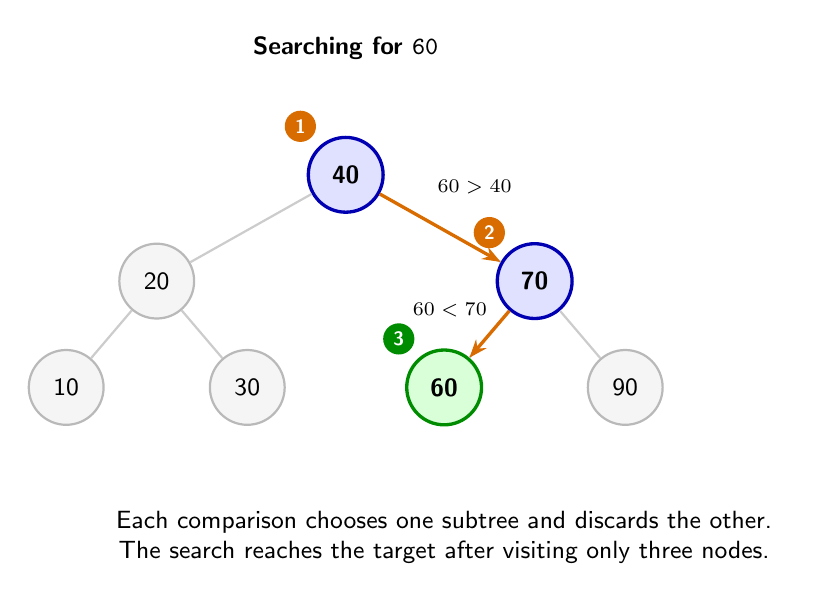
\begin{tikzpicture}[
        level distance=1.35cm,
        level 1/.style={sibling distance=4.8cm},
        level 2/.style={sibling distance=2.3cm},
        treeNode/.style={
            circle,
            draw=gray!55,
            fill=gray!8,
            minimum size=0.95cm,
            font=\sffamily\small
        },
        activeNode/.style={
            circle,
            draw=blue!70!black,
            fill=blue!12,
            very thick,
            minimum size=0.95cm,
            font=\sffamily\bfseries\small
        },
        foundNode/.style={
            circle,
            draw=green!55!black,
            fill=green!15,
            very thick,
            minimum size=0.95cm,
            font=\sffamily\bfseries\small
        },
        inactiveEdge/.style={
            draw=gray!40,
            thick
        },
        activeEdge/.style={
            -{Stealth[length=2.3mm]},
            draw=orange!85!black,
            very thick
        },
        comparisonLabel/.style={
            font=\sffamily\scriptsize,
            fill=white,
            inner sep=1.5pt
        }
    ]

        % Tree nodes
        \node[activeNode] (n40) {40}
            child[inactiveEdge] {
                node[treeNode] (n20) {20}
                child {
                    node[treeNode] (n10) {10}
                }
                child {
                    node[treeNode] (n30) {30}
                }
            }
            child[inactiveEdge] {
                node[activeNode] (n70) {70}
                child {
                    node[foundNode] (n60) {60}
                }
                child {
                    node[treeNode] (n90) {90}
                }
            };

        % Highlight the actual search path
        \draw[activeEdge]
            (n40)
            --
            node[comparisonLabel, 
            pos=0.43,
            above right,
            yshift=3mm]
            {$60 > 40$}
            (n70);

        \draw[activeEdge]
            (n70)
            --
            node[comparisonLabel,
             pos=0.42,
             above left,
             yshift=1mm]
            {$60 < 70$}
            (n60);

        % Comparison numbers
        \node[
            circle,
            fill=orange!85!black,
            text=white,
            font=\sffamily\bfseries\scriptsize,
            inner sep=1.8pt,
            above left=0.12cm and 0.08cm of n40
        ] {1};

        \node[
            circle,
            fill=orange!85!black,
            text=white,
            font=\sffamily\bfseries\scriptsize,
            inner sep=1.8pt,
            above left=0.12cm and 0.08cm of n70
        ] {2};

        \node[
            circle,
            fill=green!55!black,
            text=white,
            font=\sffamily\bfseries\scriptsize,
            inner sep=1.8pt,
            above left=0.12cm and 0.08cm of n60
        ] {3};

        % Search target
        \node[
            font=\sffamily\bfseries\small,
            above=0.85cm of n40
        ] {
            Searching for \texttt{60}
        };

        % Explanatory note
        \node[
            font=\sffamily\small,
            text width=8.7cm,
            align=center,
            below=0.95cm of n60
        ] {
            Each comparison chooses one subtree and discards the other.
            The search reaches the target after visiting only three nodes.
        };

    \end{tikzpicture}

    \caption{
        A Binary Search Tree follows only the branch that can still contain
        the target.
    }
    \label{fig:binary-search-tree-search-path}
\end{figure}

\begin{figure}[htbp]
    \centering

    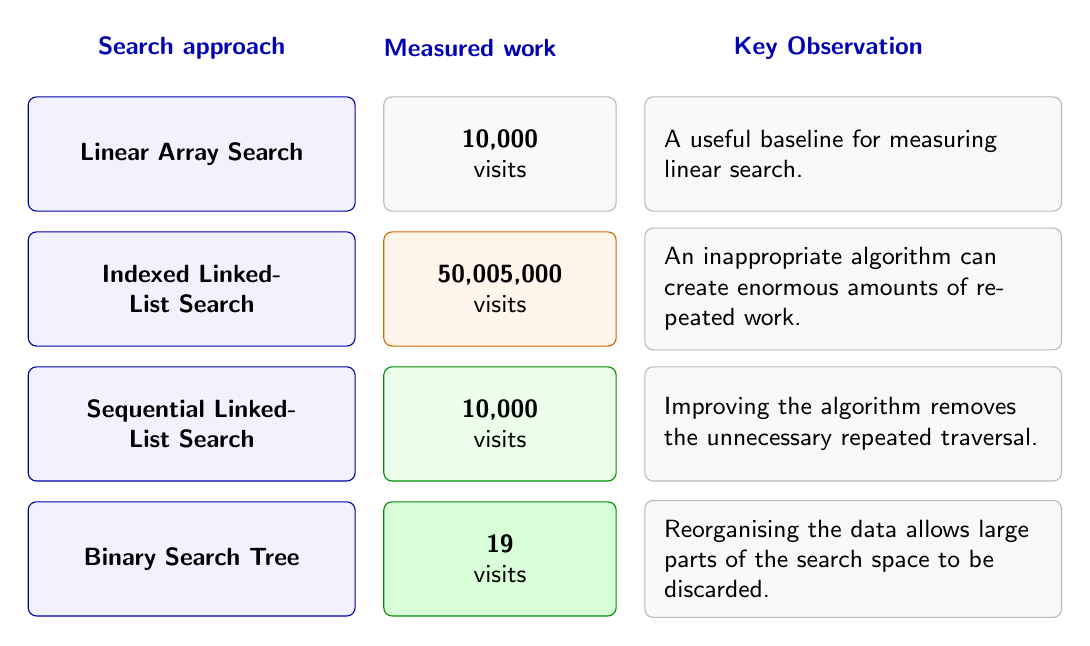
\begin{tikzpicture}[
        summaryBox/.style={
            draw=blue!65!black,
            fill=blue!5,
            rounded corners=3pt,
            minimum height=1.45cm,
            text width=3.8cm,
            align=center,
            font=\sffamily\small,
            inner sep=5pt
        },
        resultBox/.style={
            draw=gray!55,
            fill=gray!5,
            rounded corners=3pt,
            minimum height=1.45cm,
            text width=2.6cm,
            align=center,
            font=\sffamily\small,
            inner sep=5pt
        },
        lessonBox/.style={
            draw=gray!55,
            fill=gray!5,
            rounded corners=3pt,
            minimum height=1.45cm,
            text width=4.8cm,
            align=left,
            font=\sffamily\small,
            inner sep=7pt
        },
        header/.style={
            font=\sffamily\bfseries\small,
            text=blue!70!black
        }
    ]

        % Column headings
        \node[header] (methodHeader) {Search approach};
        \node[
            header,
            right=1cm of methodHeader
        ] (workHeader) {Measured work};

        \node[
            header,
            right=2cm of workHeader
        ] (lessonHeader) {Key Observation};

        % Row 1
        \node[
            summaryBox,
            below=0.35cm of methodHeader
        ] (arrayMethod) {
            \textbf{Linear Array Search}
        };

        \node[
            resultBox,
            right=0.35cm of arrayMethod
        ] (arrayWork) {
            \textbf{10,000}\\
            visits
        };

        \node[
            lessonBox,
            right=0.35cm of arrayWork
        ] (arrayLesson) {
            A useful baseline for measuring linear search.
        };

        % Row 2
        \node[
            summaryBox,
            below=0.25cm of arrayMethod
        ] (indexedMethod) {
            \textbf{Indexed Linked-List Search}
        };

        \node[
            resultBox,
            right=0.35cm of indexedMethod,
            draw=orange!80!black,
            fill=orange!8
        ] (indexedWork) {
            \textbf{50,005,000}\\
            visits
        };

        \node[
            lessonBox,
            right=0.35cm of indexedWork
        ] (indexedLesson) {
            An inappropriate algorithm can create enormous amounts of
            repeated work.
        };

        % Row 3
        \node[
            summaryBox,
            below=0.25cm of indexedMethod
        ] (sequentialMethod) {
            \textbf{Sequential Linked-List Search}
        };

        \node[
            resultBox,
            right=0.35cm of sequentialMethod,
            draw=green!55!black,
            fill=green!8
        ] (sequentialWork) {
            \textbf{10,000}\\
            visits
        };

        \node[
            lessonBox,
            right=0.35cm of sequentialWork
        ] (sequentialLesson) {
            Improving the algorithm removes the unnecessary repeated
            traversal.
        };

        % Row 4
        \node[
            summaryBox,
            below=0.25cm of sequentialMethod
        ] (treeMethod) {
            \textbf{Binary Search Tree}
        };

        \node[
            resultBox,
            right=0.35cm of treeMethod,
            draw=green!55!black,
            fill=green!15
        ] (treeWork) {
            \textbf{19}\\
            visits
        };

        \node[
            lessonBox,
            right=0.35cm of treeWork
        ] (treeLesson) {
            Reorganising the data allows large parts of the search space
            to be discarded.
        };

    \end{tikzpicture}

    \caption{
        Summary of the four search investigations performed during the
        practical.
    }
    \label{fig:search-investigation-summary}
\end{figure}


%%%%%%%%%%%%%%%%%%%%%%%%%%%%%%%%%%%%%%%%%%%%%%%%%%%%%%%%%%%%%%%%%%%%%%%%%%%%%%%%
% Engineering Takeaway
%%%%%%%%%%%%%%%%%%%%%%%%%%%%%%%%%%%%%%%%%%%%%%%%%%%%%%%%%%%%%%%%%%%%%%%%%%%%%%%%

\subsection{Engineering Takeaway}

This practical has demonstrated that efficient software is rarely achieved by
blindly replacing one data structure with another.

Instead, effective software engineering follows a process:

\begin{enumerate}
    \item measure the behaviour;
    \item identify unnecessary work;
    \item improve the algorithm;
    \item only then consider whether a different data structure is required.
\end{enumerate}

By the end of this investigation, you have seen that the organisation of data
can have a profound influence on the work an algorithm must perform.

Choosing an appropriate data structure is therefore one of the most important
design decisions a software engineer can make.

%%%%%%%%%%%%%%%%%%%%%%%%%%%%%%%%%%%%%%%%%%%%%%%%%%%%%%%%%%%%%%%%%%%%%%%%%%%%%%%%
% Challenge Activities
%%%%%%%%%%%%%%%%%%%%%%%%%%%%%%%%%%%%%%%%%%%%%%%%%%%%%%%%%%%%%%%%%%%%%%%%%%%%%%%%

\subsection{Further Investigations}

If you have completed all the required tasks, try one or more of the following
extensions to deepen your understanding of Binary Search Trees.

\begin{challengebox}
\textbf{Challenge 1: Measuring Tree Height}

Implement a function that returns the height of a Binary Search Tree.

Once complete, measure the height of the tree created from the supplied book
catalogue.

How does the height compare with the number of books stored in the tree?
\end{challengebox}

\begin{challengebox}
\textbf{Challenge 2: Does Insertion Order Matter?}

Repeat the experiment using the same books, but insert them in ascending order
of their identifiers.

Measure:

\begin{itemize}
    \item the height of the resulting tree;
    \item the amount of work required to search for the final book.
\end{itemize}

Compare your results with those produced by the original dataset.

Can you explain why the amount of work has changed?
\end{challengebox}

\begin{challengebox}
\textbf{Challenge 3: Balanced Binary Search Trees}

Your experiments may have revealed that Binary Search Trees are not always
perfectly balanced.

Research one self-balancing tree structure, such as an AVL Tree or a
Red-Black Tree.

Write a short paragraph explaining:

\begin{itemize}
    \item why balanced trees were developed;
    \item how they improve searching;
    \item one disadvantage of maintaining a balanced tree.
\end{itemize}
\end{challengebox}

\end{document}
